\chapter{参考：クロスドメイン技術候補抽出研究の図表}
\label{ch:crossdomain}

本章では、参考として、クロスドメイン技術候補抽出に関する研究で生成された図表を示す。この研究は、特許文書から課題文脈と解決手段文脈を分離し、異分野間における技術候補を抽出する手法を提案している。

\section{候補タイプの定義と実験の位置づけ}
図 \ref{fig:solution_type_quadrant} に、課題文脈類似度と解決手段文脈類似度に基づく候補タイプの概念図を示す。この図では、実験1（近接解決策型）と実験2（異質解決策型）の位置づけが明確に示されている。

\begin{figure}[htbp]
\begin{center}
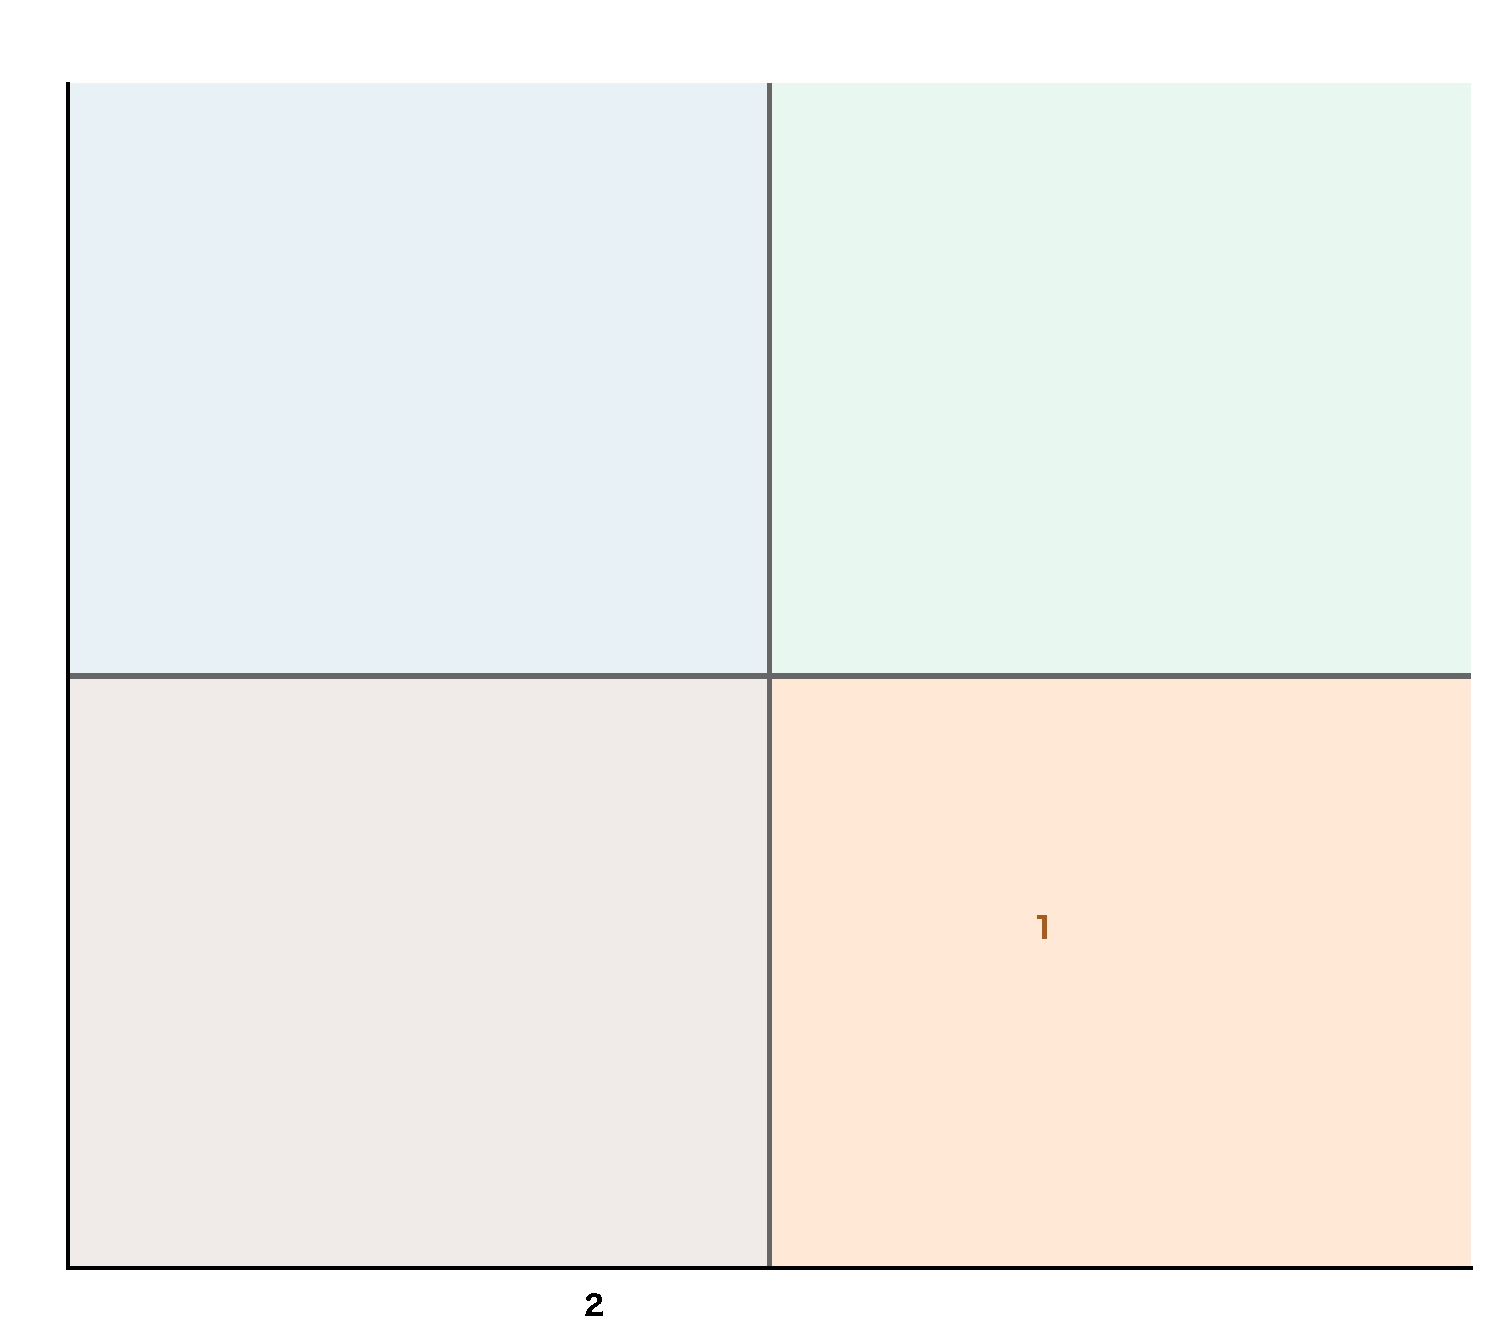
\includegraphics[width=0.85\textwidth]{./figs/solution_type_quadrant.pdf}
\caption{候補タイプと実験の位置づけ}
\label{fig:solution_type_quadrant}
\end{center}
\end{figure}

\section{提案手法の処理フロー}
図 \ref{fig:method_pipeline} に、提案手法全体の処理フローを示す。特許データから候補集合の抽出、著者確認評価に至るまでの一連のプロセスが可視化されている。

\begin{figure}[htbp]
\begin{center}
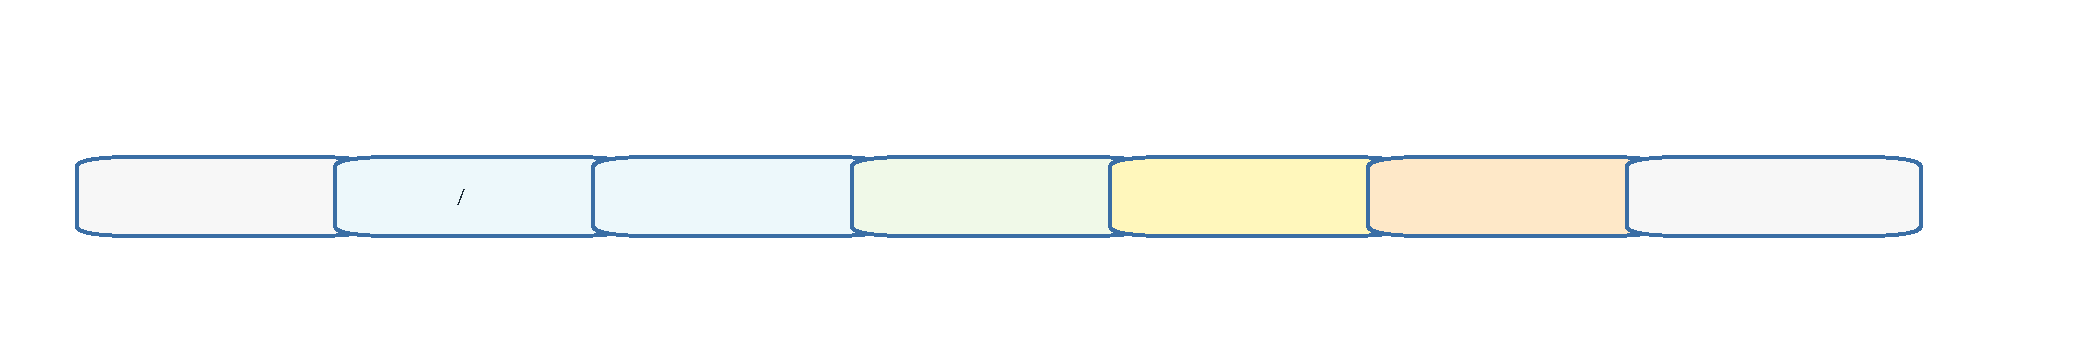
\includegraphics[width=0.95\textwidth]{./figs/method_pipeline.pdf}
\caption{提案手法の全体処理フロー}
\label{fig:method_pipeline}
\end{center}
\end{figure}

\section{実験1：U-Net候補抽出フロー}
図 \ref{fig:experiment1_pipeline} に、実験1の処理フローを示す。医療画像解析分野から製造欠陥検出分野への U-Net 関連候補抽出のプロセスが示されている。

\begin{figure}[htbp]
\begin{center}
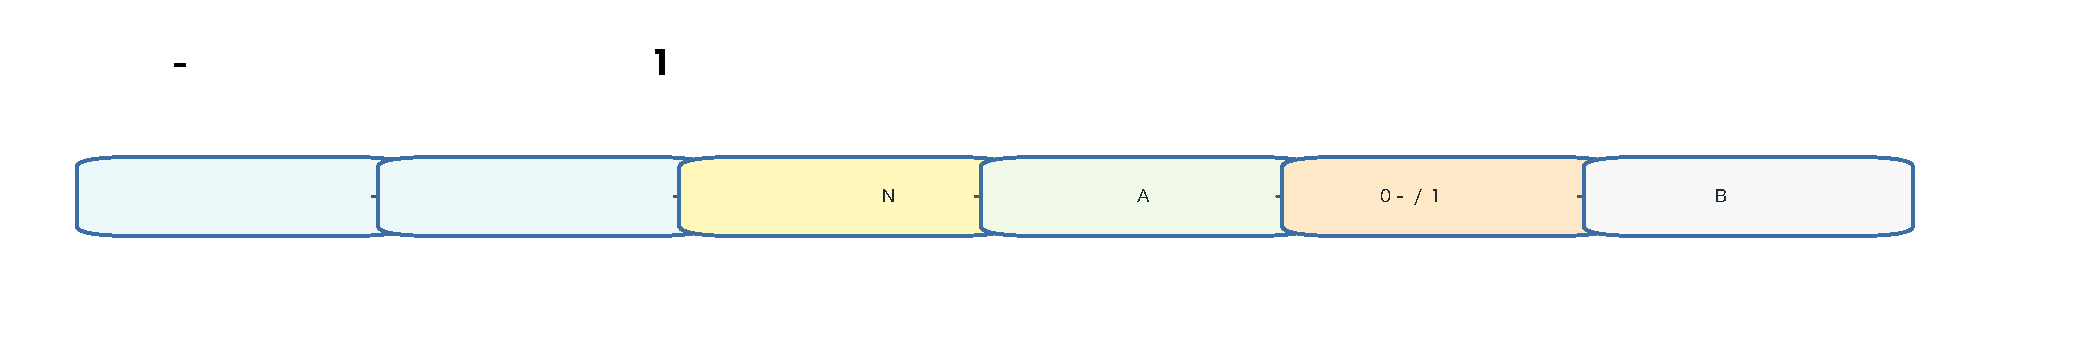
\includegraphics[width=0.95\textwidth]{./figs/experiment1_pipeline.pdf}
\caption{実験1フロー：U-Netを対象とした近接解決策型}
\label{fig:experiment1_pipeline}
\end{center}
\end{figure}

\section{実験2：異質解決策型分析フロー}
図 \ref{fig:experiment2_pipeline} に、実験2の処理フローを示す。洗浄・除去系技術を対象とした異質解決策型候補抽出のプロセスが可視化されている。

\begin{figure}[htbp]
\begin{center}
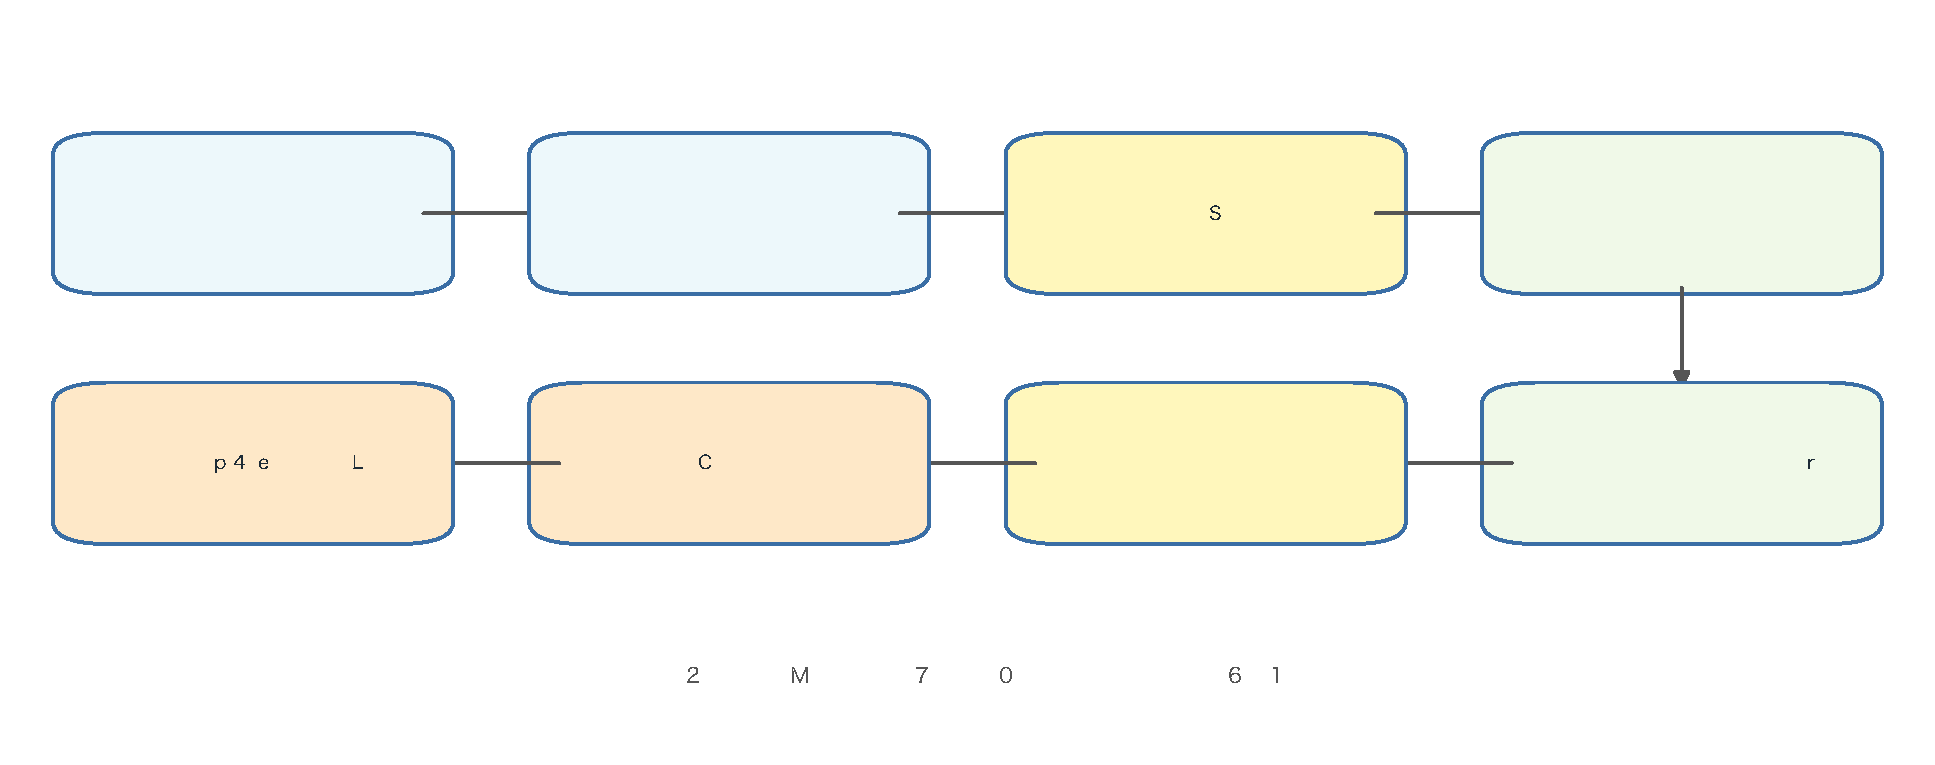
\includegraphics[width=0.95\textwidth]{./figs/experiment2_pipeline.pdf}
\caption{実験2フロー：異質解決策型の補助分析}
\label{fig:experiment2_pipeline}
\end{center}
\end{figure}

\section{実験結果}
表 \ref{tab:dataset_summary} は、実験1で使用されたデータセットのサマリーを示している。医療画像解析分野（A0）と製造欠陥検出分野（B0）におけるデータの過去・将来期間分割と U-Net の登場率が記載されている。

\begin{table}[tbp]
\centering
\small
\caption{実験1のデータセットサマリー}
\label{tab:dataset\_summary}
\begin{tabular}{llllll}
\toprule
分野 & レベル & 合計 & 過去 & 将来 & U-Net率 \\
\midrule
A0 & publication & 54100 & 10147 & 43953 & 0.030 \\
A0 & family & 30093 & 4550 & 25543 & 0.038 \\
B0 & publication & 44364 & 4307 & 40057 & 0.007 \\
B0 & family & 28450 & 2231 & 26219 & 0.008 \\
\bottomrule
\end{tabular}
\end{table}


表 \ref{tab:experiment1_results} に、実験1の著者確認評価結果を示す。提案手法による候補抽出の有効性が複数の指標で検証されている。

\begin{table}[tbp]
\centering
\small
\caption{実験1の著者確認評価サマリー}
\label{tab:experiment1\_results}
\begin{tabular}{lllll}
\toprule
グループ & 件数 & 平均スコア & 妥当性率 & 代表的フラグ \\
\midrule
baseline & 90 & 1.63 & 0.533 & 34 \\
baseline\_random & 10 & 2.20 & 0.800 & 6 \\
proposed & 43 & 1.53 & 0.465 & 16 \\
\bottomrule
\end{tabular}
\end{table}


表 \ref{tab:experiment1_baseline_comparison} に、提案手法と全文類似上位ベースラインの比較結果を示す。候補タイプ別の評価結果が整理されている。

\begin{table}[tbp]
\centering
\small
\caption{実験1ベースライン比較}
\label{tab:experiment1\_baseline\_comparison}
\begin{tabular}{llllllll}
\toprule
候補タイプ & 件数 & 平均スコア & 妥当性率 & 強い & 妥当 & 弱い & 不適切 \\
\midrule
frequency\_top\_baseline & 30 & 2.27 & 0.767 & 17 & 6 & 5 & 2 \\
fulltext\_low\_rank\_baseline & 10 & 2.20 & 0.800 & 4 & 4 & 2 & 0 \\
fulltext\_top\_baseline & 30 & 0.567 & 0.167 & 1 & 4 & 6 & 19 \\
future\_growth & 10 & 1.10 & 0.300 & 2 & 1 & 3 & 4 \\
proposed\_top & 23 & 1.61 & 0.522 & 5 & 7 & 8 & 3 \\
true\_random\_baseline & 30 & 2.07 & 0.667 & 16 & 4 & 6 & 4 \\
unet\_related & 10 & 1.80 & 0.500 & 4 & 1 & 4 & 1 \\
\bottomrule
\end{tabular}
\end{table}


表 \ref{tab:experiment2_label_summary} に、実験2の評価ラベル分布を示す。異質解決策型における候補の解釈可能性が確認されている。

\begin{table}[tbp]
\centering
\small
\caption{実験2評価ラベルサマリー}
\label{tab:experiment2\_label\_summary}
\begin{tabular}{ll}
\toprule
ラベル & 件数 \\
\midrule
◎ 強い候補 & 11 \\
○ 妥当候補 & 5 \\
△ 弱い候補 & 12 \\
× 不適切候補 & 18 \\
\bottomrule
\end{tabular}
\end{table}


表 \ref{tab:experiment2_cluster_summary} に、実験2のクラスタレベル評価結果を示す。各クラスタにおける候補品質が分析されている。

\begin{table}[tbp]
\centering
\small
\caption{実験2クラスタレベルの評価サマリー}
\label{tab:experiment2\_cluster\_summary}
\begin{tabular}{llllllll}
\toprule
クラスタ & 件数 & 強い & 妥当 & 弱い & 不適切 & 強い/妥当率 & 広い候補率 \\
\midrule
adhesive\_cleaning & 7 & 2 & 0 & 0 & 5 & 0.286 & 0.286 \\
circuit\_board\_cleaning & 3 & 1 & 1 & 1 & 0 & 0.667 & 1.000 \\
cmp\_polishing\_post\_cleaning & 12 & 0 & 0 & 5 & 7 & 0.000 & 0.417 \\
flux\_electronic\_component\_cleaning & 5 & 1 & 1 & 2 & 1 & 0.400 & 0.800 \\
photoresist\_resin\_mask\_removal & 6 & 2 & 0 & 2 & 2 & 0.333 & 0.667 \\
semiconductor\_substrate\_cleaning & 6 & 5 & 1 & 0 & 0 & 1.000 & 1.000 \\
silicon\_wafer\_cleaning & 7 & 0 & 2 & 2 & 3 & 0.286 & 0.571 \\
\bottomrule
\end{tabular}
\end{table}


表 \ref{tab:experiment_comparison} に、実験1と実験2の評価結果の比較を示す。主分析と補助分析の性質の違いが明確に表れている。

\begin{table}[tbp]
\centering
\small
\caption{実験1と実験2の評価結果比較}
\label{tab:experiment\_comparison}
\begin{tabular}{lllll}
\toprule
実験 & 評価ユニット数 & 平均スコア & 妥当件数 & 妥当性率 \\
\midrule
実験1 & 143 & 1.64 & 76 & 0.531 \\
実験2 & 46 & 1.20 & 16 & 0.348 \\
\bottomrule
\end{tabular}
\end{table}

